\documentclass{amsart}
\synctex=1

%=================================================================
% 
\newcount\DraftStatus  % 0 suppresses notes to selves in text
\DraftStatus=1   % TODO: set to 0 for final version
%=================================================================

%=================================================================
\usepackage{comment}
%=================================================================
%
\includecomment{JournalOnly}  
\includecomment{ConferenceOnly}  
\includecomment{TulipStyle}
%
%=================================================================
\input{preamble}


%=================================================================
%
\begin{document}
%
%=================================================================
%
\title[Learning Process]{Kaggle Project Report}%

\author{PengCheng Jiang}
\address[A.~1]{School of Computer Science,\\ 
JiLin University, jilin 130000, China}%
\email[A.~1]{pcjiang@tulip.academy}

\author{Gang Li}
\address[A.~2]{School of Information Technology \\
Deakin University, Geelong, VIC 3216, Australia}%
\email[A.~2]{gang.li@deakin.edu.au}



%\thanks{Thanks to \ldots}%
\subjclass{Artificial Intelligence}%
\date{\gitAuthorDate}%


\begin{abstract}
    This week,I studied kaggle,slides,notebook
\end{abstract}

\keywords{kaggle,slides,notebook}%




\maketitle
\tableofcontents

\newpage
%=================================================================

%=================================================================
\section{Problem Definition}
Last year, in the Toxic Comment Classification Challenge, you built multi-headed models to recognize toxicity and several subtypes of toxicity. This year's competition is a related challenge: building toxicity models that operate fairly across a diverse range of conversations.

Here’s the background: When the Conversation AI team first built toxicity models, they found that the models incorrectly learned to associate the names of frequently attacked identities with toxicity. Models predicted a high likelihood of toxicity for comments containing those identities (e.g. "gay"), even when those comments were not actually toxic (such as "I am a gay woman"). This happens because training data was pulled from available sources where unfortunately, certain identities are overwhelmingly referred to in offensive ways. Training a model from data with these imbalances risks simply mirroring those biases back to users.

In this competition, you're challenged to build a model that recognizes toxicity and minimizes this type of unintended bias with respect to mentions of identities. You'll be using a dataset labeled for identity mentions and optimizing a metric designed to measure unintended bias. Develop strategies to reduce unintended bias in machine learning models, and you'll help the Conversation AI team, and the entire industry, build models that work well for a wide range of conversations.
\section{Text preprocessing}
\begin{itemize}
  \item Count the total number of words contained in all texts, the maximum and minimum number of words contained in a text
  \item Check for missing data
  \item Change abbreviations to full:isn't -> is not(via dictionnary)
  \item clean_numbers
  \item Find all non alphabetic characters and clean_special_chars
  \item Solve the problem of misspelling words
  \item lower
\end{itemize}
\par
\begin{figure}[h]
  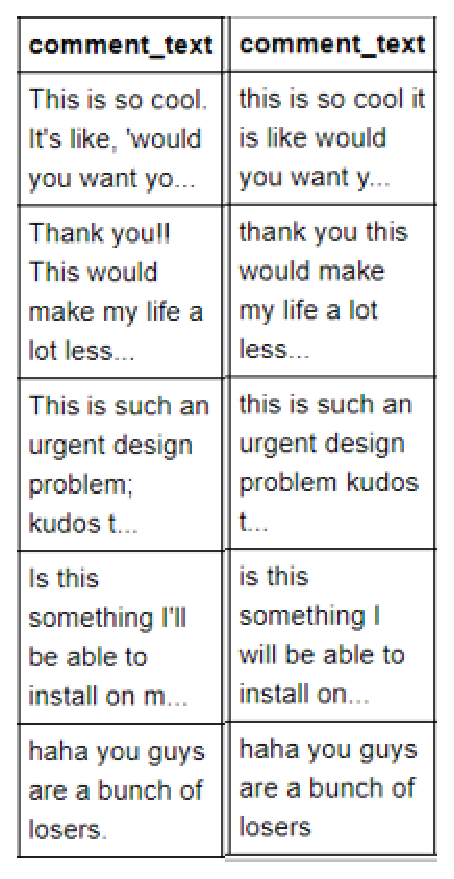
\includegraphics[scale=0.5]{picture/result.eps}
  \caption{data cleaning}\label{fig:1}
\end{figure}
\section{Embedding}
\begin{itemize}
  \item What tokenizer does is actually very simple. It divides the words it sees into spaces, and then uses numbers to correspond one by one. Then we take the first num_ Words is the word with the highest frequency, others are not recognized.
  \item First learn the dictionary of the text, and then get the corresponding relationship between words and numbers, and then convert the text into a number string through this relationship, and then use the padding method to make up the number string to the same degree, then you can proceed to the next step : embedding
  \item collections.counter,pytorch:torchtext.vocab,
  \item The embedding layer is the same as word2vec. Whether it is skip gram or cbow model, they infer each other from the context and the current, so we consider the relationship between the preceding and the following. 
  \item glove.42B.300d.txt
\end{itemize}
\section{module}
\begin{itemize}
  \item Long short term memory (LSTM) is a special RNN, which is mainly used to solve the problem of gradient disappearance and gradient explosion in the process of long sequence training. In short, LSTM can perform better in longer sequences than ordinary RNN
  \item BiRNN:In practical problems, there are also problems that not only rely on the previous sequence, but also rely on the subsequent sequence for prediction. For those problems, we need to use bidirectional RNN (birnn)
  \item embed_size, num_hiddens, num_layers = 300, 100, 2
\end{itemize}
\begin{center}
  \begin{figure}
    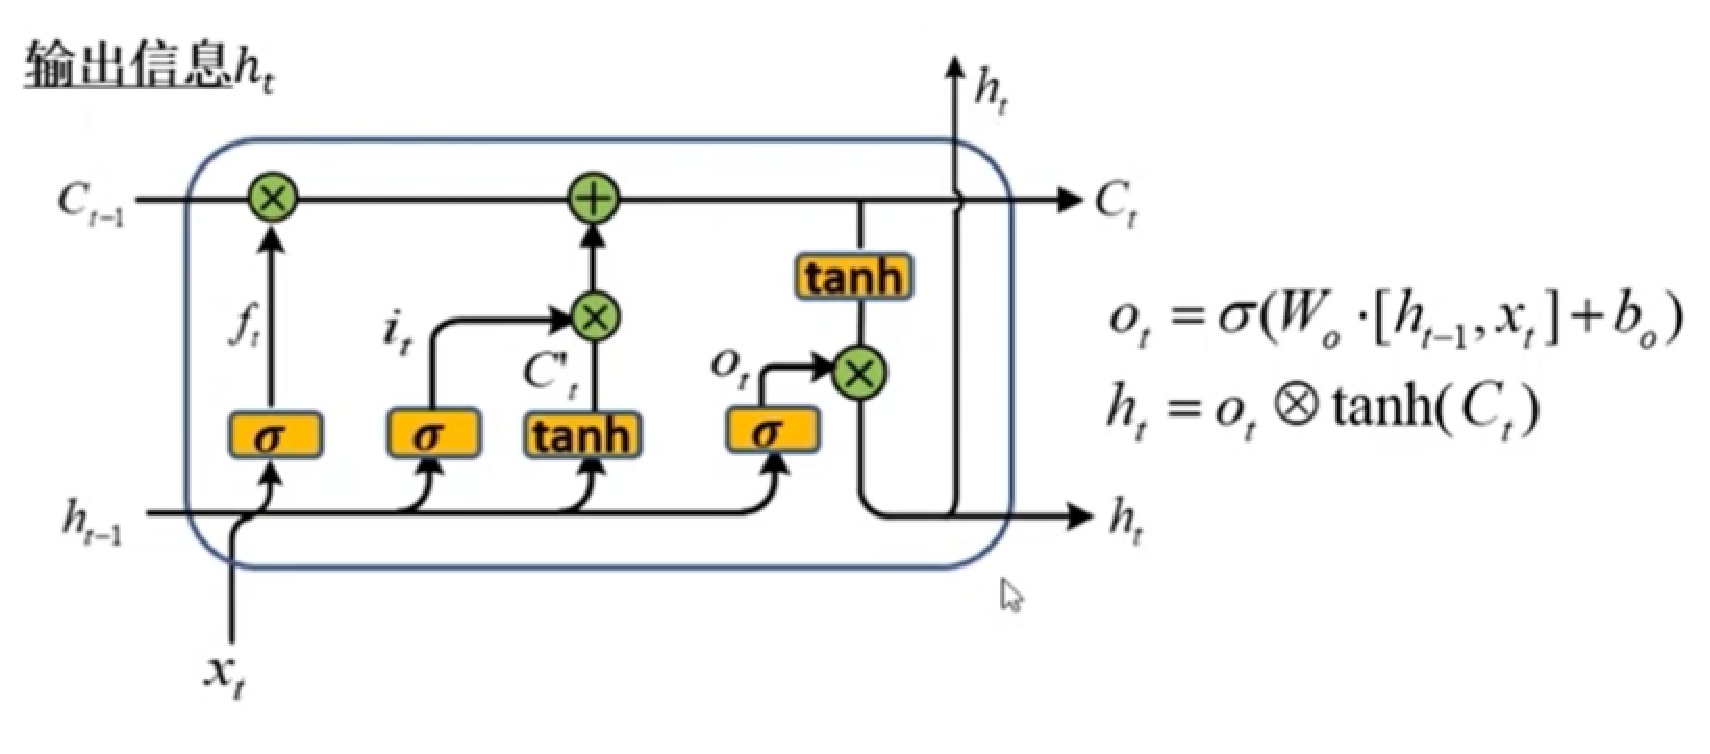
\includegraphics[scale=0.5]{picture/lstm.eps}
    \caption{LSTM}\label{fig:2}
  \end{figure}
\end{center}
\begin{center}
  \begin{figure}
    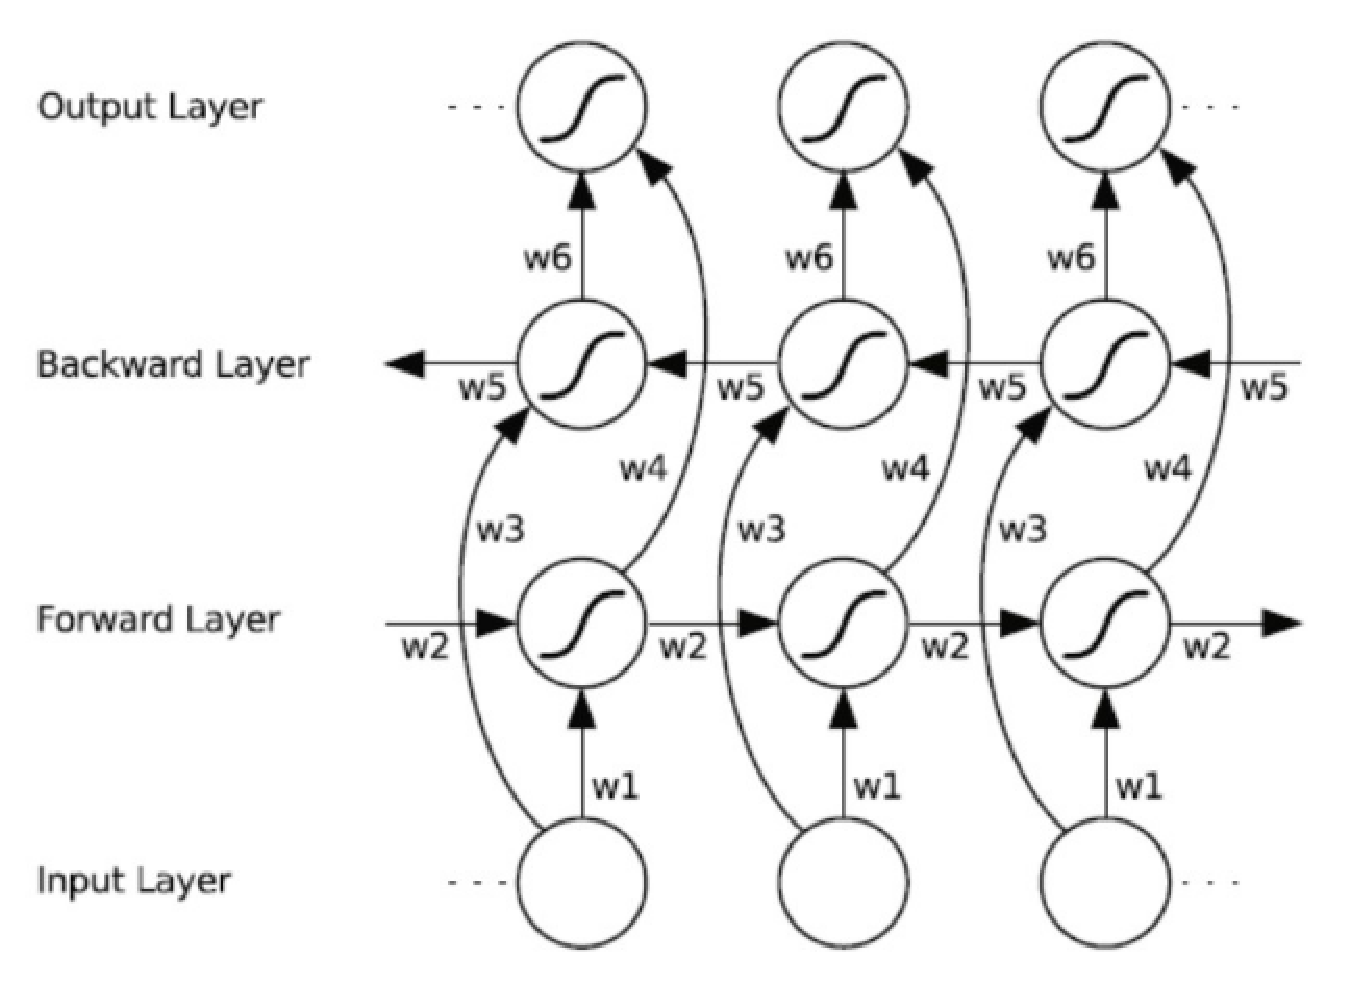
\includegraphics[scale=0.5]{picture/birnn.eps}
    \caption{BIRNN}\label{fig:3}
  \end{figure}
\end{center}
\section{Conlusion}
Through text processing and glove embedding, the model achieves good results



\end{document}

